\documentclass[11pt]{article}
\usepackage[letterpaper,left=0.9in,right=0.9in,top=1in,bottom=1in]{geometry}
\usepackage{libertinus}\usepackage{amsmath}
\usepackage{xcolor}\usepackage{tikz}
\usetikzlibrary{arrows.meta,positioning,calc,fit,backgrounds,shadows.blur}
\definecolor{accent}{HTML}{2E86AB}
\definecolor{deep}{HTML}{1B5A78}
\definecolor{muted}{HTML}{6B7C88}
\pagestyle{empty}

% A stack, drawn as a stack: the engine is the foundation at the bottom and the
% tint lightens as you go up. Every concrete item is a chip, chained with
% `right=of` so the widths look after themselves.
\tikzset{
  slab/.style ={draw=accent!55, line width=0.7pt, rounded corners=4pt,
                minimum width=13.9cm, minimum height=2.80cm, anchor=south west},
  bar/.style  ={draw=none, rounded corners=1.5pt, anchor=south west,
                minimum width=3.6pt, minimum height=2.80cm},
  chip/.style ={draw=accent!45, line width=0.5pt, fill=white, rounded corners=2.5pt,
                font=\scriptsize, inner xsep=4.4pt, inner ysep=0pt, anchor=west,
                text height=1.55ex, text depth=0.45ex, minimum height=4.6mm},
  idx/.style  ={font=\scriptsize\sffamily\bfseries, text=white},
  nm/.style   ={font=\large\sffamily\bfseries, text=deep, anchor=base west},
  role/.style ={font=\small\itshape, text=muted, anchor=base west},
  how/.style  ={font=\scriptsize\ttfamily, text=muted, anchor=base east},
  owns/.style ={font=\scriptsize, text=deep, anchor=west},
  dep/.style  ={draw=accent, line width=1.1pt, -{Stealth[length=5.5pt,width=4.5pt]}},
  deplab/.style={font=\scriptsize\ttfamily, text=accent, fill=white, inner sep=1.8pt},
}
\newcommand{\ow}[1]{{\scriptsize\color{muted}owns\;}#1}

\begin{document}
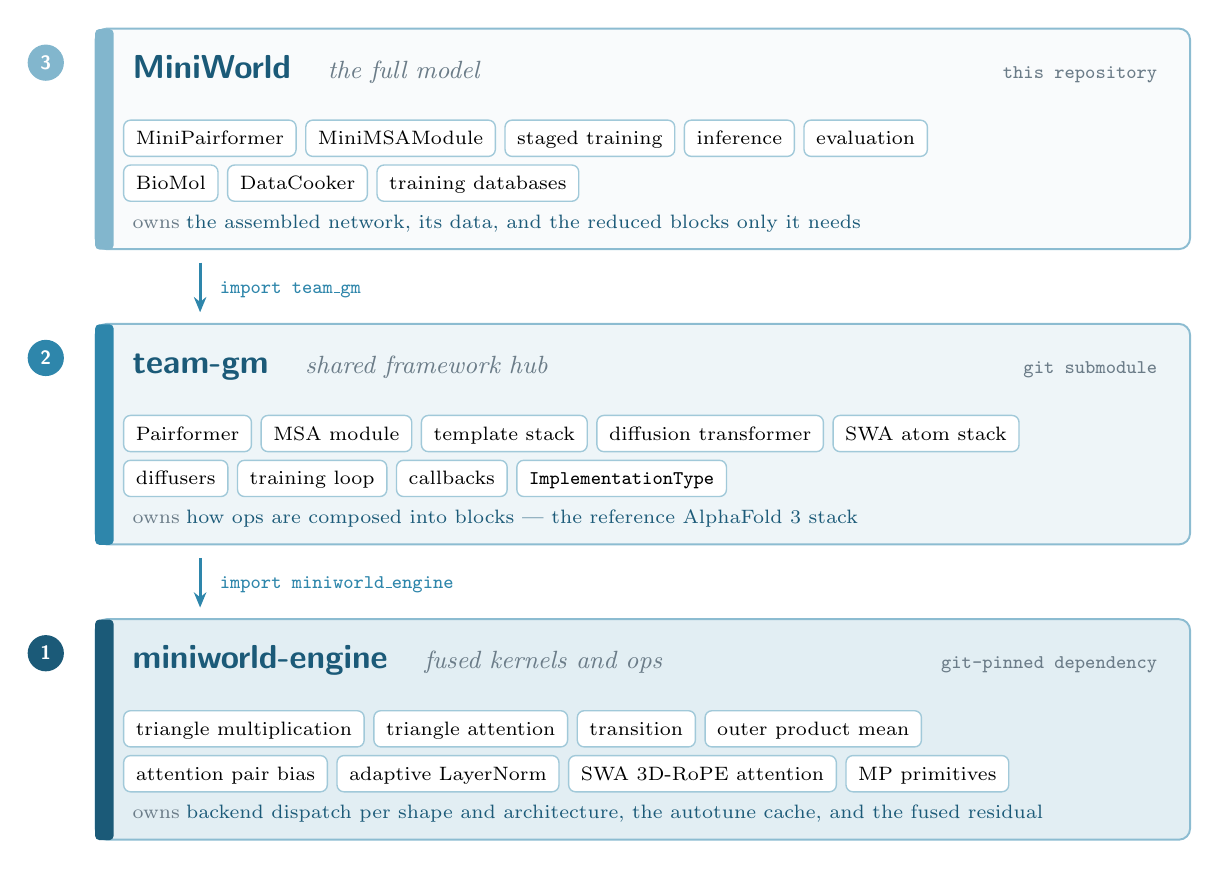
\begin{tikzpicture}[x=1cm,y=1cm]
  \def\L{0.95}      % slab left edge
  \def\R{14.85}     % slab right edge
  \def\H{2.80}

  % ---------------------------------------------------------------- slabs
  % bottom = foundation. Tint darkens downward.
  \node[slab, fill=accent!14] (eng) at (\L,0)        {};
  \node[slab, fill=accent!8 ] (gm)  at (\L,3.75)     {};
  \node[slab, fill=accent!3 ] (mw)  at (\L,7.50)     {};
  \node[bar, fill=deep]        at (\L,0)     {};
  \node[bar, fill=accent]      at (\L,3.75)  {};
  \node[bar, fill=accent!60]   at (\L,7.50)  {};

  % layer index discs
  \foreach \y/\c/\n in {0/deep/1, 3.75/accent/2, 7.50/accent!60/3}
    \node[circle, fill=\c, minimum size=4.6mm, inner sep=0pt, idx] at (\L-0.62,\y+\H-0.42) {\n};

  % ---------------------------------------------------------------- layer 3
  \node[nm]   (mwn)  at (\L+0.36, 7.50+\H-0.62) {MiniWorld};
  \node[role]        at ($(mwn.base east)+(0.22,0)$) {the full model};
  \node[how]         at (\R-0.28, 7.50+\H-0.62) {this repository};
  \node[chip] (m1) at (\L+0.36, 7.50+\H-1.38) {MiniPairformer};
  \node[chip, right=3pt of m1] (m2) {MiniMSAModule};
  \node[chip, right=3pt of m2] (m3) {staged training};
  \node[chip, right=3pt of m3] (m4) {inference};
  \node[chip, right=3pt of m4] (m5) {evaluation};
  \node[chip] (m6) at (\L+0.36, 7.50+\H-1.95) {BioMol};
  \node[chip, right=3pt of m6] (m7) {DataCooker};
  \node[chip, right=3pt of m7] (m8) {training databases};
  \node[owns] at (\L+0.36, 7.50+0.34)
        {\ow{the assembled network, its data, and the reduced blocks only it needs}};

  % ---------------------------------------------------------------- layer 2
  \node[nm]   (gmn)  at (\L+0.36, 3.75+\H-0.62) {team-gm};
  \node[role]        at ($(gmn.base east)+(0.22,0)$) {shared framework hub};
  \node[how]         at (\R-0.28, 3.75+\H-0.62) {git submodule};
  \node[chip] (g1) at (\L+0.36, 3.75+\H-1.38) {Pairformer};
  \node[chip, right=3pt of g1] (g2) {MSA module};
  \node[chip, right=3pt of g2] (g3) {template stack};
  \node[chip, right=3pt of g3] (g4) {diffusion transformer};
  \node[chip, right=3pt of g4] (g5) {SWA atom stack};
  \node[chip] (g6) at (\L+0.36, 3.75+\H-1.95) {diffusers};
  \node[chip, right=3pt of g6] (g7) {training loop};
  \node[chip, right=3pt of g7] (g8) {callbacks};
  \node[chip, right=3pt of g8] (g9) {\texttt{ImplementationType}};
  \node[owns] at (\L+0.36, 3.75+0.34)
        {\ow{how ops are composed into blocks --- the reference AlphaFold~3 stack}};

  % ---------------------------------------------------------------- layer 1
  \node[nm]   (en)   at (\L+0.36, 0+\H-0.62) {miniworld-engine};
  \node[role]        at ($(en.base east)+(0.22,0)$) {fused kernels and ops};
  \node[how]         at (\R-0.28, 0+\H-0.62) {git-pinned dependency};
  \node[chip] (e1) at (\L+0.36, 0+\H-1.38) {triangle multiplication};
  \node[chip, right=3pt of e1] (e2) {triangle attention};
  \node[chip, right=3pt of e2] (e3) {transition};
  \node[chip, right=3pt of e3] (e4) {outer product mean};
  \node[chip] (e5) at (\L+0.36, 0+\H-1.95) {attention pair bias};
  \node[chip, right=3pt of e5] (e6) {adaptive LayerNorm};
  \node[chip, right=3pt of e6] (e7) {SWA 3D-RoPE attention};
  \node[chip, right=3pt of e7] (e8) {MP primitives};
  \node[owns] at (\L+0.36, 0+0.34)
        {\ow{backend dispatch per shape and architecture, the autotune cache, and
         the fused residual}};

  % ---------------------------------------------------------------- deps
  % dependency runs downward: MiniWorld imports team-gm imports the engine
  \draw[dep] (\L+1.34, 7.50-0.16) -- (\L+1.34, 3.75+\H+0.16);
  \node[deplab, anchor=west] at (\L+1.52, 7.50-0.50) {import team\_gm};
  \draw[dep] (\L+1.34, 3.75-0.16) -- (\L+1.34, 0+\H+0.16);
  \node[deplab, anchor=west] at (\L+1.52, 3.75-0.50) {import miniworld\_engine};
\end{tikzpicture}
\end{document}
